\documentclass[12pt,a4paper]{paper}
\usepackage[utf8]{inputenc}
\usepackage[english]{babel}
\usepackage{amsmath}
\usepackage{enumitem}
\usepackage{amsfonts}
\usepackage{amssymb}
\usepackage[left=2cm,right=2cm,top=2cm,bottom=2cm]{geometry}
\usepackage{Sweave}
\begin{document}
\title{STAT646 - Exam 2\\\small{Daniel Osorio - dcosorioh@tamu.edu\\Department of Veterinary Integrative Biosciences\\Texas A\&M University}}
\maketitle
\Sconcordance{concordance:Osorio_Daniel_E2.tex:Osorio_Daniel_E2.Rnw:%
1 8 1 1 0 5 1 1 2 1 0 1 3 2 0 2 1 1 3 5 0 1 2 1 1 1 2 4 0 1 2 1 1 1 2 1 %
0 1 1 4 0 2 2 1 0 2 1 4 0 2 2 1 0 4 1 8 0 1 3 6 0 1 3 6 0 1 3 7 0 1 2 1 %
1 1 2 1 0 2 1 5 0 1 1 1 3 6 0 1 2 2 1 1 2 1 0 4 1 3 0 1 2 1 1 1 2 1 0 1 %
1 1 10 9 0 3 1 16 0 1 2 1 1 1 2 1 0 1 1 4 0 2 2 7 0 1 2 3 1}

\begin{enumerate}
\item The `exam2\_data1' data attached in the email are read counts from a next-gen sequencing (RNA-Seq) experiment on humans under two conditions (three healthy individuals and three diseased individuals).
\begin{Schunk}
\begin{Sinput}
> library("DESeq2")
> data1 <- read.csv(file = "exam2_data1.csv", 
+                   stringsAsFactors = FALSE, 
+                   row.names = 1)
> colData <- data.frame(Status=as.factor(rep(x = c("N","Y"),each=3)))
> nbData <- cbind(colData,t(data1))
> data1 <- DESeqDataSetFromMatrix(countData = data1, 
+                                 colData = colData, 
+                                 design = ~ Status)
\end{Sinput}
\end{Schunk}
\begin{enumerate}
\item Use the rlog function from the DESeq2 package to transform the read counts. Using the rlog-transformed counts:
\begin{Schunk}
\begin{Sinput}
> rlogData <- assay(rlog(data1))
\end{Sinput}
\end{Schunk}
\begin{enumerate}
\item Carry out cluster analysis to explore structure among the assays (columns). Interpret the results. \textit{There is not a clear structure in the data separating individuals by status, healthy and diseased individuals are all mixed in the reported clusters.}
\begin{Schunk}
\begin{Sinput}
> par(mar=c(4,3,1,1), mgp=c(1.5,0.5,0))
> plot(hclust(dist(t(rlogData))))
\end{Sinput}
\end{Schunk}
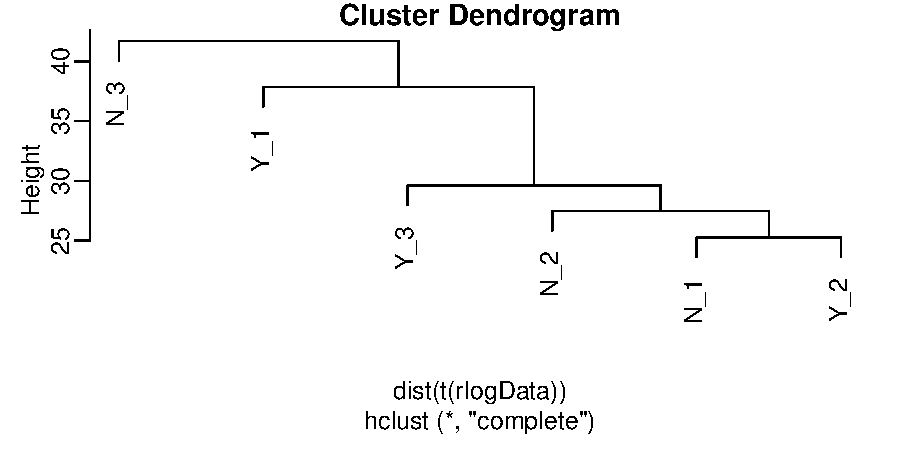
\includegraphics{Osorio_Daniel_E2-003}
\item Carry out principal component analysis to explore structure among the assays (columns). Interpret the results. \textit{As in the hierarchical clustering, healthy and diseased individuals are all mixed, showing that there is not a clear structure in the data separating individuals by status.}
\begin{Schunk}
\begin{Sinput}
> par(mar=c(3,3,1,1), mgp=c(1.5,0.5,0))
> outData <- prcomp(t(rlogData), center = TRUE, scale. = TRUE)$x
> plot(outData, col= colData$Status, pch=16)
\end{Sinput}
\end{Schunk}
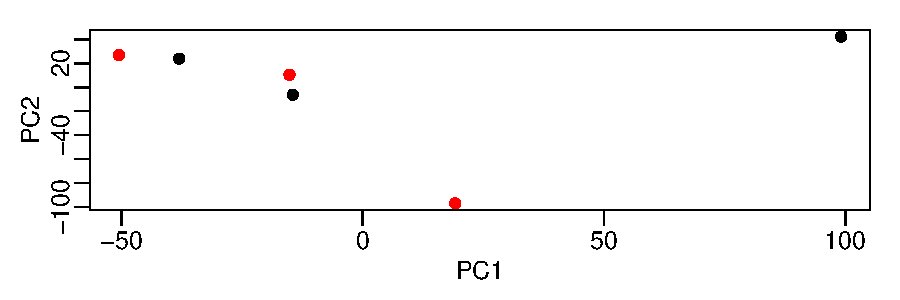
\includegraphics{Osorio_Daniel_E2-004}
\item Use naïve Bayes to classify training individuals as diseased or healthy, using all 10,525 genes as predictor variables. Report a confusion matrix. What are the following estimated values: classification accuracy rate, sensitivity, specificity. You do not have to use cross validation or set aside any data for testing purposes. That said, how would you expect cross validation or test-set estimates of accuracy, sensitivity, and specificity to compare to the ones you reported? \textit{Expected results of cross-validation or test-set estimates of accuracy, sensitivity, and specificity should be lower in value than the reported ones, that is due the model could be overfitted to the actual dataset and perform poorly classifying new datasets.}
\begin{Schunk}
\begin{Sinput}
> library(e1071)
> nbResults <- naiveBayes(Status ~., data = nbData)
> nbPredict <- predict(nbResults, newdata = nbData[,-1])
> cMatrix <- table(Observed = colData$Status,Predicted = nbPredict)
> cMatrix
\end{Sinput}
\begin{Soutput}
        Predicted
Observed N Y
       N 3 0
       Y 0 3
\end{Soutput}
\begin{Sinput}
> # Accuracy
> (cMatrix[1,1] + cMatrix[2,2])/sum(cMatrix)
\end{Sinput}
\begin{Soutput}
[1] 1
\end{Soutput}
\begin{Sinput}
> # Sensitivity
> cMatrix[2,2]/sum(cMatrix[2,])
\end{Sinput}
\begin{Soutput}
[1] 1
\end{Soutput}
\begin{Sinput}
> # Specificity
> cMatrix[1,1]/sum(cMatrix[1,])
\end{Sinput}
\begin{Soutput}
[1] 1
\end{Soutput}
\end{Schunk}
\end{enumerate}
\item Use the DESeq function from the DESeq2 package to perform differential expression analysis. How many genes are selected at an FDR of 0.05 as being different between disease and healthy individuals? Use the plotCounts function to plot the normalized read counts (not raw read counts) for the top-ranked gene (the one with the smallest associated FDR estimate).
\begin{Schunk}
\begin{Sinput}
> deResults <- DESeq(data1)
> deResults <- results(deResults, pAdjustMethod = "fdr")
> sum(deResults$padj <= 0.05, na.rm = TRUE)
\end{Sinput}
\begin{Soutput}
[1] 1
\end{Soutput}
\begin{Sinput}
> par(mar=c(3,3,1,1), mgp=c(2,0.5,0))
> plotCounts(data1, gene = "Gene_321", las = 1, pch = 16, 
+            normalized = TRUE,intgroup = "Status", 
+            col= colData$Status)
\end{Sinput}
\end{Schunk}
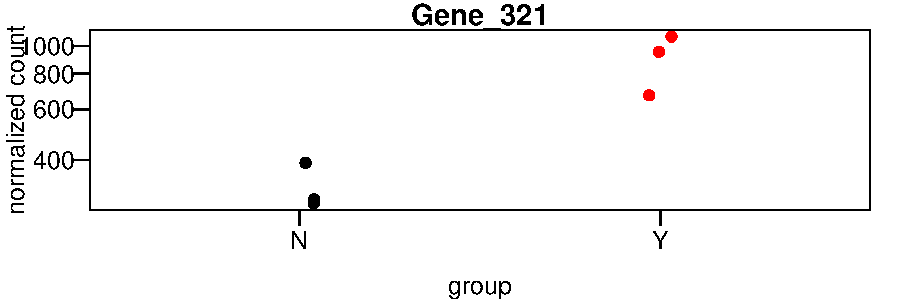
\includegraphics{Osorio_Daniel_E2-006}
\end{enumerate}
\item Consider an RNA-seq experiment in which we are comparing a treatment group to a control group. Let $Y_{ijk}$ be the read count for gene $k$ in sample i of comparison group $j$, $i = 1, 2,\dots$, $n_{j}$ , j = 1, \dots, m. What would be wrong with assuming that $Y_{ijk} \sim Poisson(\lambda_{jk})$ \textit{Under the assumption of Poisson distribution, we are assuming that for a given gene, the mean and the variance are the same, this event doesn't apply for RNA-seq data. RNA-seq data follows a negative binomial distribution with different variances associated with genes having the same mean. Under the Poisson distribution assumption, we will overestimate the differences in gene expression between the two samples.}
\item Context = `exam2\_data2.csv' These are simulated, continuous -omics data. There are 2,000 features and 300 samples, with 100 samples each in three classes. In the data file, the first 75 samples are to be used as training samples for class A, the next 75 samples are to be used as training samples for class B, etc. So, the first 225 samples are training data. The last 75 samples are test data. The first 25 of these are for class A, the next 25 for class B, etc.
\begin{Schunk}
\begin{Sinput}
> data2 <- read.csv("exam2_data2.csv", row.names = 1)
> trainingData <- t(data2[,1:225])
> testingData <- t(data2[,226:300])
> trainingClass <- as.factor(gsub("_[[:digit:]]+","",rownames(trainingData)))
> testingClass <- as.factor(gsub("_[[:digit:]]+","",rownames(testingData)))
\end{Sinput}
\end{Schunk}
\begin{enumerate}
\item Classify with KNN. Consider values of $K = 1, 2, \dots, 10$. Compute the test error for each value.
\begin{Schunk}
\begin{Sinput}
> library(class)
> K <- 1:10
> ACC <- sapply(K, function(k){
+   set.seed(1)
+   predictedClass <- knn(train = trainingData, 
+                       test = testingData, 
+                       cl = trainingClass, 
+                       k = k)
+ outKNN <- table(Observed = testingClass, 
+                 Predicted = predictedClass)
+ sum(diag(outKNN))/sum(outKNN)
+ })
> testError <- round(1-ACC,2)
> names(testError) <- paste0("K= ",K)
> cbind(testError)
\end{Sinput}
\begin{Soutput}
      testError
K= 1       0.33
K= 2       0.37
K= 3       0.36
K= 4       0.33
K= 5       0.28
K= 6       0.28
K= 7       0.29
K= 8       0.27
K= 9       0.29
K= 10      0.24
\end{Soutput}
\end{Schunk}
\begin{enumerate}
\item Provide a plot with K on the x-axis and test accuracy on the y-axis. Interpret the plot.
\begin{Schunk}
\begin{Sinput}
> par(mar=c(3,3,1,1), mgp=c(2,0.5,0))
> plot(K, ACC, ylim = c(0,1), pch = 16, type = "b")
\end{Sinput}
\end{Schunk}
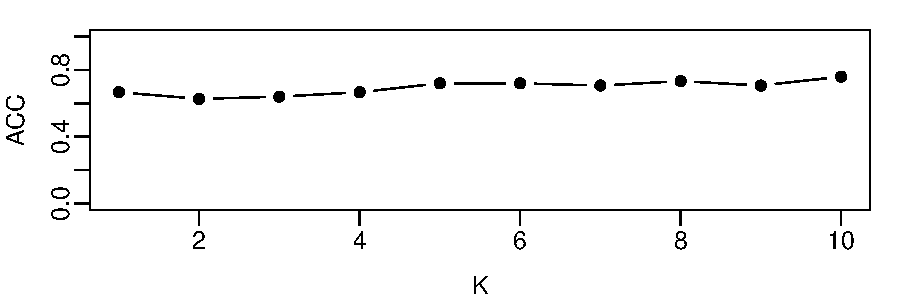
\includegraphics{Osorio_Daniel_E2-009}
\item Which value of K achieves the highest test accuracy, and what is that accuracy?
\begin{Schunk}
\begin{Sinput}
> K[which.max(ACC)]
\end{Sinput}
\begin{Soutput}
[1] 10
\end{Soutput}
\end{Schunk}
\end{enumerate}
\end{enumerate}
\end{enumerate}
\end{document}
